
\section{Pipeline Specification}

In {\Builder}, the digital twin (DT) pipeline is described using the Function+Data Flow (FDF)~\cite{decontoFunction+DataFlowFramework2024} domain-specific language. We summarize FDF as implemented in {\Builder}. 

FDF support four categories of boxes, based on FDF. These boxes can be selected on the Library, available either on the left side on the UI or also accessible by right clickin on the canvas:

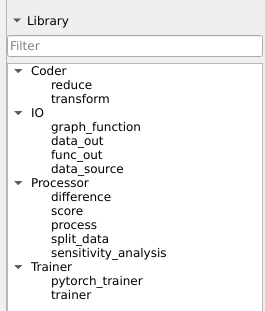
\includegraphics[width=0.3\textwidth]{lib.png}

\begin{itemize}
    \item Coder for model order reduction by learning an encoding/decoding function
    with unsupervised learning algorithms (e.g., principal component analysis),
    \item IO (Input/Output) for general input/output, i.e., to represent the pipeline's external dependencies, 
    \item Processor for typical data processing by reusing functions learned by other
    boxes, as well as predefined functions.
    \item Trainer for data assimilation by learning a function with supervised ML (e.g.,
    a neural network learned with gradient descent).
\end{itemize}

The boxes can have several input and output ports. There are two types of ports:
\begin{itemize}
    \item Function ports (in {\color{red}red}) for sending/receiving a single {\em learned function},
    \item Data ports (in black) for sending/receiving a batch of data. 
\end{itemize}

\subsection{Processor Boxes}

Processor boxes are represented by a light blue rectangle and it has multiple \IDP s to receive the data for processing, and multiple \ODP s to return the processed data. 
The rectangle is used is the most typical shape used in a flowchart. 

The function to execute can be:
\begin{itemize}
    \item Provided through an \IFP~(function learned by the previous boxes) and is implemented with a \verb|process| box; \\
    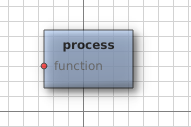
\includegraphics[width=0.3\textwidth]{proc.png}
    \item A predefined function from the {\Builder} library.
\end{itemize}

The following table summarizes the pre-defined functions from the Builder.

\begin{tabular}{lp{6cm}l}
	\toprule
	Name & Description & Plot \\
	\midrule
	difference & 
    Calculate the element-wise difference between two arrays. 
    & N \\
	score & 
    Compute and log various regression metrics, generate plots, and save results to files. 
    & Y \\
	split\_data & Split data into training and testing sets & N \\
	sensitivity\_analysis & Given a ML model, determine two $\varepsilon$-close  (`x1', `x2') inputs that results in two outputs (`y1', `y2') which are significantly different. & Y \\
	\bottomrule
\end{tabular}

\subsection{Coder Boxes}

The {\em Coder boxes} are represented by a pale green trapezoid. It has multiple \IDP s to receive the data from which to compute the reduced basis and one or two \OFP s to return the encoder and decoder functions (i.e., the projection and inverse projection onto the reduced basis, respectively). 
The trapezoid is chosen to alude to the process of encoding/decoding that is implemented and in a reference to what is used, e.g., to represent variational auto-encoders. 

Two types of Coder boxes are supported: reduce and transform. 
The reduce box supports two algorithms chosen in the Box parameter:
%REMOVE "pca\_std" and include param for percentage of basis kept
\begin{itemize}
    \item \verb|std_pca|: standardization followed by PCA
    \item \verb|pca|: only PCA
\end{itemize}
In the back-end, these are implemented with Scikit-Learn.



\subsection{Trainer Boxes}
The {\em Trainer boxes} are represented by a pale violet pentagon. 
This shape is chosen with its sharp edge to indicate the single output of this box as a model. It has $\ell \geq 2$ \IDP s to receive the supervised $(X, Y)$ pairs, with $k < \ell$ ports providing $X$ and the remaining $k'=\ell-k$ providing $Y$, and it has one \OFP~ to return a function that predicts $Y$ given $X$. The number $k$ is provided in the first component of the Trainer box parameter. The Trainer boxes have no \IFP: the specific ML training algoritm is specified by the type of trainer and associated parameters, as described next. 

Two types of trainer are supported: \verb|trainer| and \verb|pytorch_trainer|. The \verb|trainer| exposes a number of scikit-learn algorithms:
\begin{itemize}
    \item support vector regression (svr)
    \item decision tree (dt)
    \item multi-layer perceptron (mlp)
    \item linear regression (lr)
\end{itemize}

\verb|pytorch_trainer| allow for more sophisticated pytorch-based multi-layer
perceptron neural network. It allows to easily configure learning parameters
such as learning rate, iterations in the learning loop, etc.

\subsection{Input/Output Boxes}

\begin{itemize}
    \item \verb|data_source|: load a data from disk.
    The following format are supported: 
    \begin{itemize}
        \item comma-separated values (CSV) ".csv"
        \item python Pickle ".pickle"
        \item Matlab mat7.3 format ".mat" (loaded using mat73 python library)
    \end{itemize}
    \item \verb|func_out|: save a function to be reused in other pipeline. The function is saved in the pickle format.
\end{itemize}

\section{User Interface}

The {\Builder} user interface provides access to all essential parameters of the DT pipeline within a single workspace. It consists of the following components:
\begin{itemize}
    \item a \emph{canvas} to create the various boxes and interconnect their ports. 
    Users can connect ports via drag-and-drop. %(linking the output of one box to the input of another).
    Function connections are depicted in red, while data connections are black. Implicit type checking is automatically triggered with each new connection to help ensure correctness. Once the ports are connected, their types are propagated throughout the pipeline.
    \item a \emph{library selector} to create new boxes as required,
    \item a \emph{parameter editor} to edit parameters of the selected box (e.g., adjust neural network learning parameters),
    \item A \verb|Run| button to trigger the pipeline execution. 
\end{itemize}

\includegraphics[width=0.9\textwidth]{builder-ui.png}

When the \verb|Run| button is clicked, the pipeline is exported to the execution back-end and executed. The run results results are displayed on the Output panel.
%
The execution back-end and other pipeline parameters can be configured in the  Settings button (
\includegraphics[height=0.8\baselineskip]{settings.png}). 
%
Validation metrics and plots are displayed by clicking on the charts panel (
\includegraphics[height=0.8\baselineskip]{charts.png}). This panel is only clickable if a box with charts/metrics output, such as \verb|sensitivity_analysis| is selected:

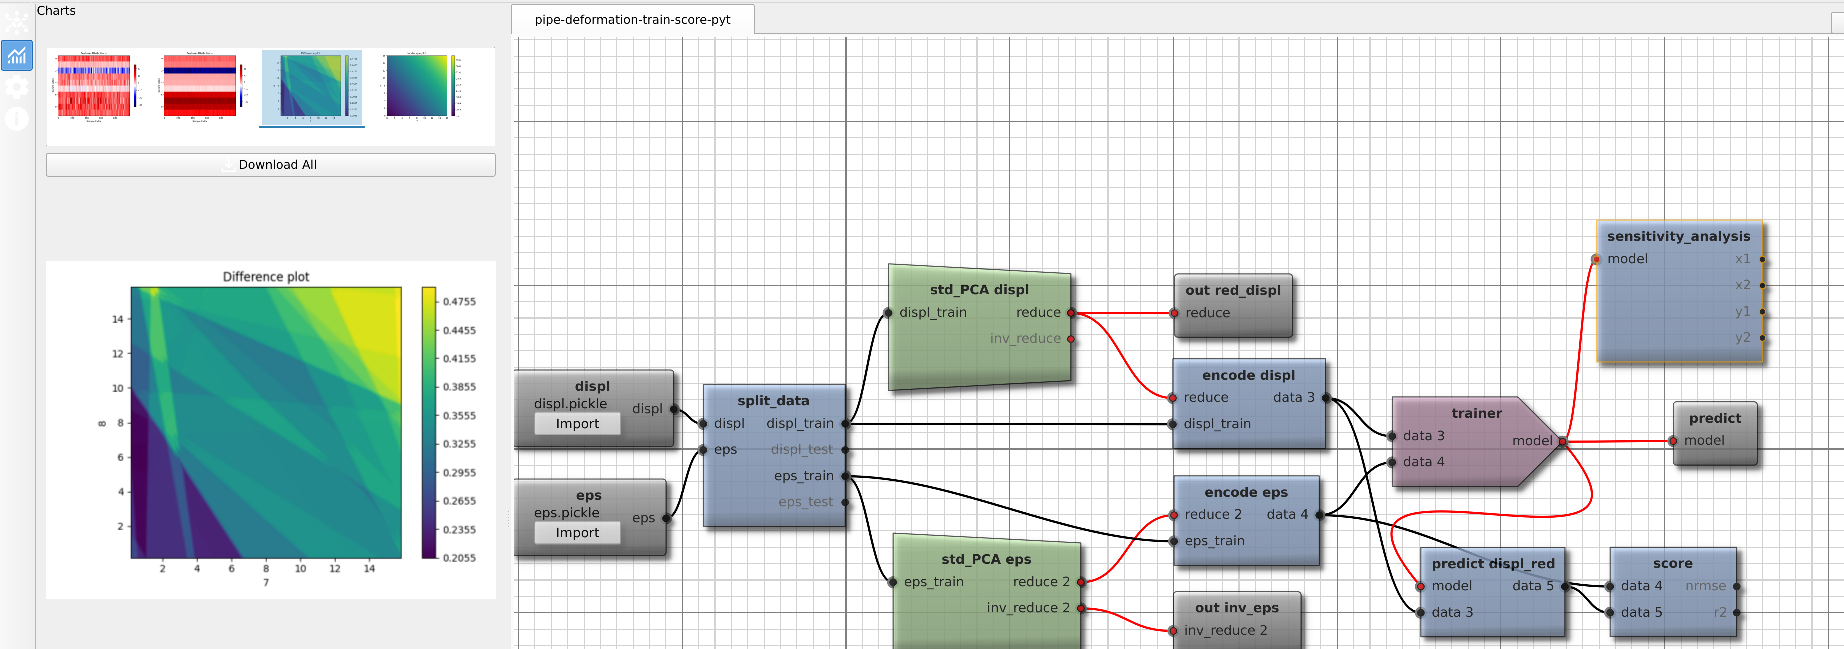
\includegraphics[width=0.9\textwidth]{plot_display.png}

\section{User Workflow}

{\Builder} workflow has three main steps: specify the pipeline, run the pipeline to produce the different models and data, and analyze the results for validation. \\

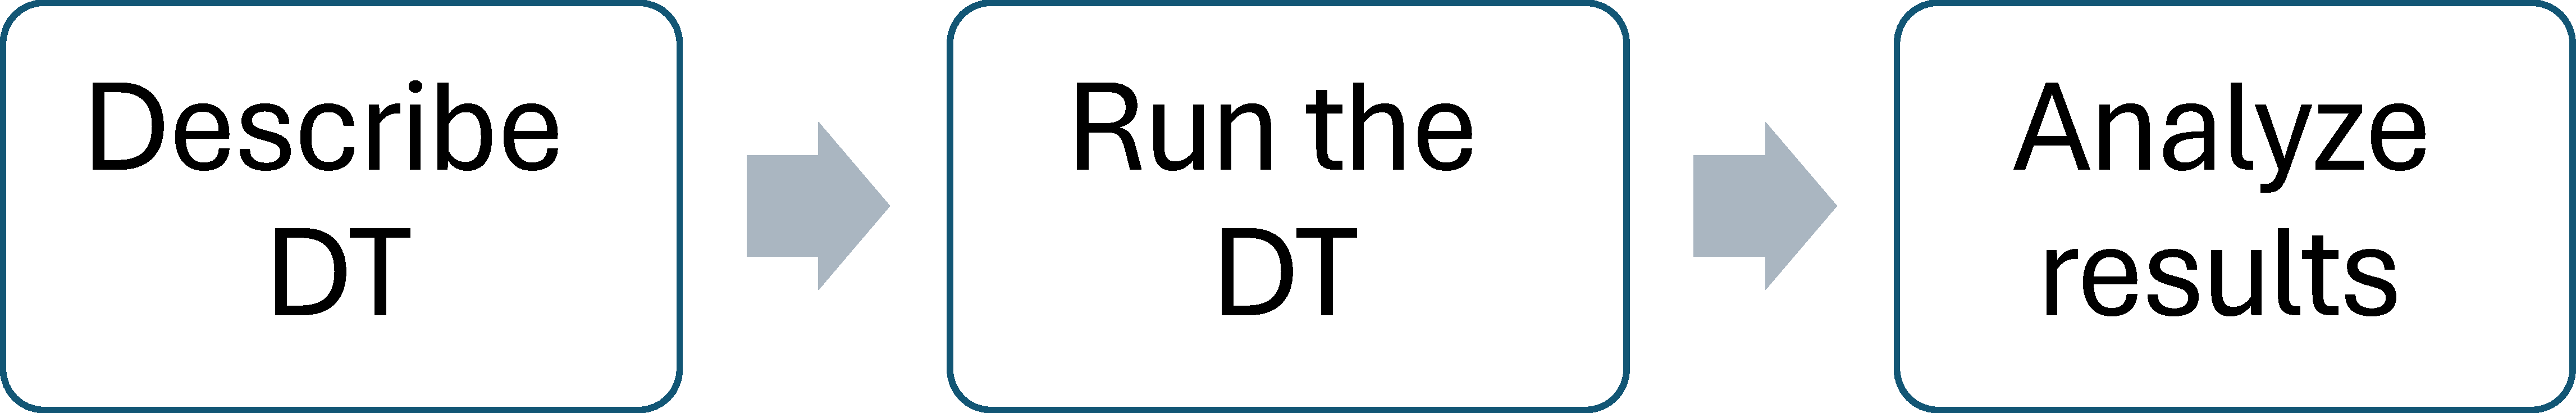
\includegraphics[width=0.9\textwidth]{flow_builder.pdf}

\paragraph{Step 1. Specify the Pipeline.}

This step involves describing the twinning pipeline using boxes and interconnecting them as required. Boxes can be added by selecting them in the Library and the connections can be done by dragging and drop ports.
%
To facilitate the description and ensure the correctness of the pipeline, {\Builder} performs several automated checks, offering immediate feedback to the user during the pipeline's creation and interconnection. Specifically, the tool ensures that the pipeline is \emph{always syntactically correct}, e.g.\ by ensuring that an output port can only be connected to input ports of the same class (Data or Function). For example, connecting an output data port to an input function port is forbidden. Data ports are indicated by a black filled circle (\tikz\draw[black,fill=black] (0,0) circle (.5ex);) and function ports by a red filled circle (\tikz\draw[black,fill=red] (0,0) circle (.5ex);).

\emph{Implicit typing} is also implemented. A warning may be triggered when connecting two data ports:

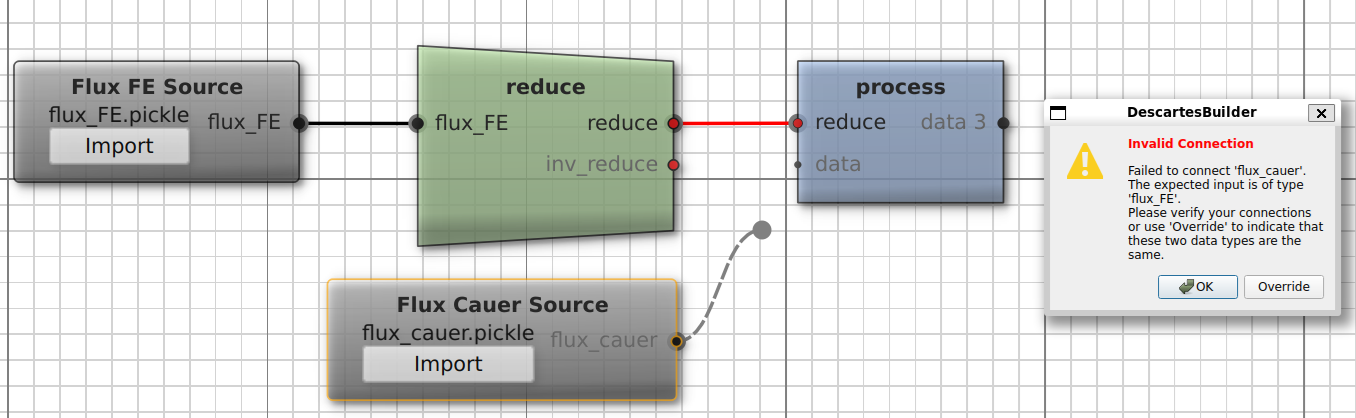
\includegraphics[width=0.9\textwidth]{3_typing.png}

This happens when the type of data connected to a Processor box does not match the expected type (as carried over by the function propagated from previous boxes, both for fixed functions from the {\Builder} library {\em and} functions learned within the pipeline \cite{decontoFunction+DataFlowFramework2024}). Overriding the warning is possible, in which case the two types are matched, and propagated throughout the pipeline, avoiding forthcoming similar warnings. 
%
Specifically, the user can either select ``OK'' and proceed to fix the pipeline or they can select ``Override'' to explicitly indicate that the two types are identical.


\paragraph{Step 2. Execute the pipeline.}
Once the user is satisfied with the pipeline, they can click on the \texttt{Run} button to trigger the execution of the pipeline. The execution consists of 
(i) exporting the pipeline and the associated parameters into the executable back-end,
and (ii) launching the back-end. After the execution, the front end collects and displays the execution results on the \texttt{Output} panel. %Currently, only a back-end based on the Kedro~\cite{alamKedro2024} library is supported. 


\paragraph{Step 3. Validate the models.}

Certain boxes produce plots and metrics useful for validating the models and data produced:

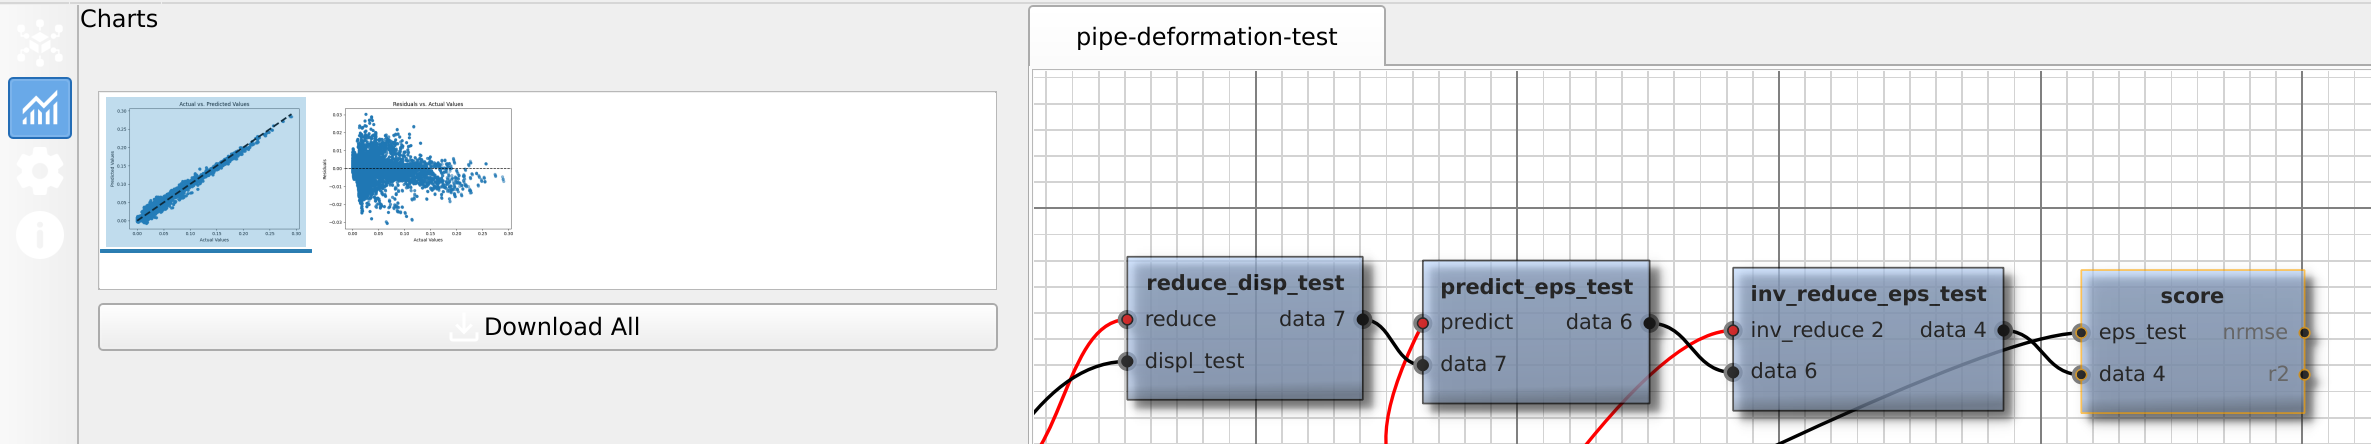
\includegraphics[width=0.9\linewidth]{4_score_box_result_alt.png}

For instance, the Score Processor box provides metrics (normalized RMSE, etc.) and diagrams (e.g.\ residual plots), to understand if a surrogate is similar enough to the original high-fidelity model.
